%----------------------------------------------------------------------------
%----------------------------------------------------------------------------
The far field diffraction pattern of a uniformly illuminated pinhole is the well known Airy function. The radial displacement $r_1$ of the first minimum some distance $z$ down the beam line is given by \cite{Saleh:1991a}
%----------------------------------------------------------------------------
\begin{equation}
r_1
=
z
\frac
{1.22\lambda}
{2r},
\end{equation}
%----------------------------------------------------------------------------
where $\lambda$ is the wavelength of the incident beam, and $r$ is the pinhole rdius. The Rayleigh range for a circular aperture is \cite{Saleh:1991a}
%----------------------------------------------------------------------------
\begin{equation}
z_R
=
\frac
{\pi r^2}
{\lambda}.
\end{equation}
%----------------------------------------------------------------------------
For distances $z>z_R$ we will assume to be in the far field limit. For the beam line in figure \ref{conditioning_table}, the pinholes (b), (e), and (h) are 0.2 m upstream from +0.2 m lenses. Suppose the pinholes have a diameter of 25 $\mu$m and consider the beam from dye laser \#21 (725 nm). The Rayleigh range for this pinhole is 677 $\mu$m; thus, the lenses are in the far field. At the lens the radial displacement of the first minimum is 7.076 mm, yielding a semi-Gaussian (by placing a 14.2 mm aperture before the +0.2 m lens) beam with a full width of about 14 mm. See figure \ref{spot_size}.
%----------------------------------------------------------------------------
% spot_size.tex
% by Troy Hix, May 2005
%----------------------------------------------------------------------------
\begin{figure}
\centering
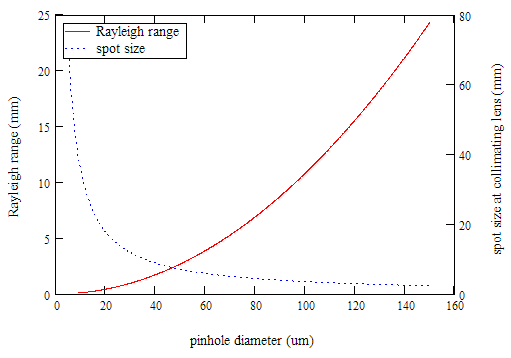
\includegraphics[width=4.00in]
{spot_size/spot_size.png}
\caption[Rayleigh range (724 nm) and spot size vs. pinhole diameter]{Rayleigh range (724 nm) and spot size vs. pinhole diameter. Even with a pinhole as large as 150 $\mu$m the Rayleigh range for the pinhole function is only 24.374 mm while the spot size 20 cm from the pinhole is 2.359 mm in diameter. For a pinhole with a diameter of 50 $\mu$m the Rayleigh range is 2.708 mm and the spot size at 20 cm is 7.076 mm.}
\label{spot_size}
\end{figure} 
%----------------------------------------------------------------------------

%----------------------------------------------------------------------------
%----------------------------------------------------------------------------
%----------------------------------------------------------------------------
\subsubsection{Damage threshold}
%----------------------------------------------------------------------------
In the following analysis we will assume the beams involved have a circular top-hat intensity distributions for simplicity.

Pinholes made to handle high power from standard suppliers typically have a damage threshold of around 1MW/mm$^2$. Given a waist at the pinhole of about 80 $\mu$m, we can only use 4.4 ns pulses with about 100 $\mu$J of energy. The ratio of the area of the pinhole to the total area of the beam implies that only 10\% of the energy incident on the pinhole makes it through. Since the central maximum of the Airy function contains about 84\% of the energy in the pinhole, the beam after the +0.2 m lens can have about 8 $\mu$J of energy at most. This 8 $\mu$J is then run through an aperture before the iodine cell. If this aperture has a radius of around 1 mm then the energy of the beam at the iodine sample is about 160 nJ. This is 2 to 3 orders of magnitude less than our estimate of the energy needed at the iodine sample for coherent control. Thus, an ordinary metallic pinhole may not be the best choice. A glass fiber will be better: the only limit is the surface damage threshold of the glass: around 5GW/cm$^2$. See figure \ref{energy}.
%----------------------------------------------------------------------------
% energy.tex
% by Troy Hix, May 2005
%----------------------------------------------------------------------------
\begin{figure}
\centering
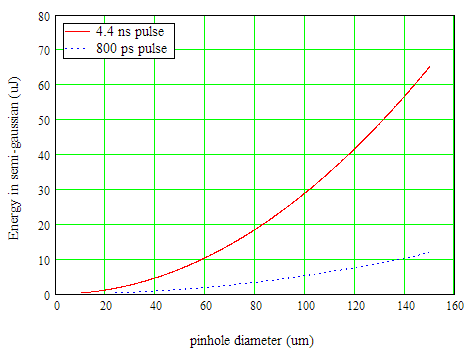
\includegraphics[width=4.00in]
{energy/energy.png}
\caption{Energy in the Airy function central max vs. pinhole size.}
\label{energy}
\end{figure} 
%----------------------------------------------------------------------------

%----------------------------------------------------------------------------
%----------------------------------------------------------------------------
%----------------------------------------------------------------------------
